%%%% Paramétrage du cours %%%%
\def\xxactivite{Cours}

\fichefalse \proftrue \tdfalse \courstrue

\def\xxnumchapitre{Chapitre 1 \vspace{.2cm}}
\def\xxchapitre{\hspace{.12cm} Découverte de l'algorithmique et de la programmation}

\def\xxcompetences{%
\textsl{%
\textbf{Savoirs et compétences :}\\
\begin{itemize}[label=\ding{112},font=\color{bleuxp}] 
\item Choisir un type de variable.
\item Concevoir un algorithme utilisant une structure conditionnelle (Si), une structure itérative (while), une structure itérative (for).
\item Concevoir une fonction.
\item  Manipuler des listes.
\item Instruction et expression.
\end{itemize}
}}

\def\xxfigures{
%\includegraphics[width=\linewidth]{matlab}
%\\
%\textit{Modèle du pilote hydraulique avec pilotage interactif.}
}%figues de la page de garde

\input{\repRel/Style/pagegarde_cours_minitoc}
\setlength{\columnseprule}{.1pt}

\vspace{2cm}
\pagestyle{fancy}
\thispagestyle{plain}

%%%%%%%%%%%%%%%%%%%%%%%


\section{Avant-Propos}
\subsection{Définitions}

\begin{defi}{Informatique -- Wikipedia}
L'informatique est un domaine d'activité scientifique, technique, et industriel concernant le traitement automatique de l'information numérique par l'exécution de programmes informatiques hébergés par des dispositifs électriques-électroniques : des systèmes embarqués, des ordinateurs, des robots, des automates, etc.
\end{defi}

\begin{defi}{Algorithmique -- Wikipedia}
Un algorithme est une méthode générale pour résoudre un type de problèmes. Il est dit correct lorsque, pour chaque instance du problème, il se termine en produisant la bonne sortie, c'est-à-dire qu'il résout le problème posé.
\end{defi}

L'efficacité d'un algorithme est mesurée notamment par :
\begin{itemize}
\item sa durée de calcul ;
\item sa consommation de mémoire vive (en partant du principe que chaque instruction a un temps d'exécution constant) ;
\item la précision des résultats obtenus (par exemple avec l'utilisation de méthodes probabilistes) ;
\item sa scalabilité (son aptitude à être efficacement parallélisé) ;
\item etc.
\end{itemize}

Les ordinateurs sur lesquels s'exécutent ces algorithmes ne sont pas infiniment rapides, car le temps de machine reste une ressource limitée, malgré une augmentation constante des performances des ordinateurs. Un algorithme sera donc dit performant s'il utilise avec parcimonie les ressources dont il dispose, c'est-à-dire le temps CPU, la mémoire vive et (aspect objet de recherches récentes) la consommation électrique. L’analyse de la complexité algorithmique permet de prédire l'évolution en temps calcul nécessaire pour amener un algorithme à son terme, en fonction de la quantité de données à traiter.

\begin{defi}{Programmation -- Wikipedia}
La programmation, appelée aussi codage dans le domaine informatique, désigne l'ensemble des activités qui permettent l'écriture des programmes informatiques. C'est une étape importante du développement de logiciels.

L'écriture d'un programme se fait dans un langage de programmation. Un logiciel est un ensemble de programmes (qui peuvent être écrits dans des langages de programmation différents) dédié à la réalisation de certaines tâches par un (ou plusieurs) utilisateurs du logiciel.

\end{defi}

La programmation représente donc ici la rédaction du code source d'un logiciel. On utilise plutôt le terme développement pour dénoter l'ensemble des activités liées à la création d'un logiciel et des programmes qui le composent. Cela inclut la spécification du logiciel, sa conception, puis son implémentation proprement dite au sens de l'écriture des programmes dans un langage de programmation bien défini, ainsi que la vérification de sa correction, etc.

\subsection{Environnement de développement}
Pour répondre à un problème informatique, on pourra réfléchir à l'algorithme permettant de le résoudre. Une des premières approches consiste donc à utiliser un papier et un crayon pour proposer une réponse structurée au problème.

Il faudra ensuite traduire cet algorithme dans un langage de programmation. Nous utiliserons pour cela \texttt{Python}.

Pour programmer en \texttt{Python} il est nécessaire d'utiliser un éditeur de texte (pour écrire le code) et un interpréteur pour exécuter le code. 
En règle générale, on utilise pour cela un environnement de développement (IDE). On pourra \textbf{Pyzo} ou \textbf{Spyder} (ou tout autre environnement vous paraissant satisfaisant). 

\begin{figure}[H]
\centering
%\begin{center}
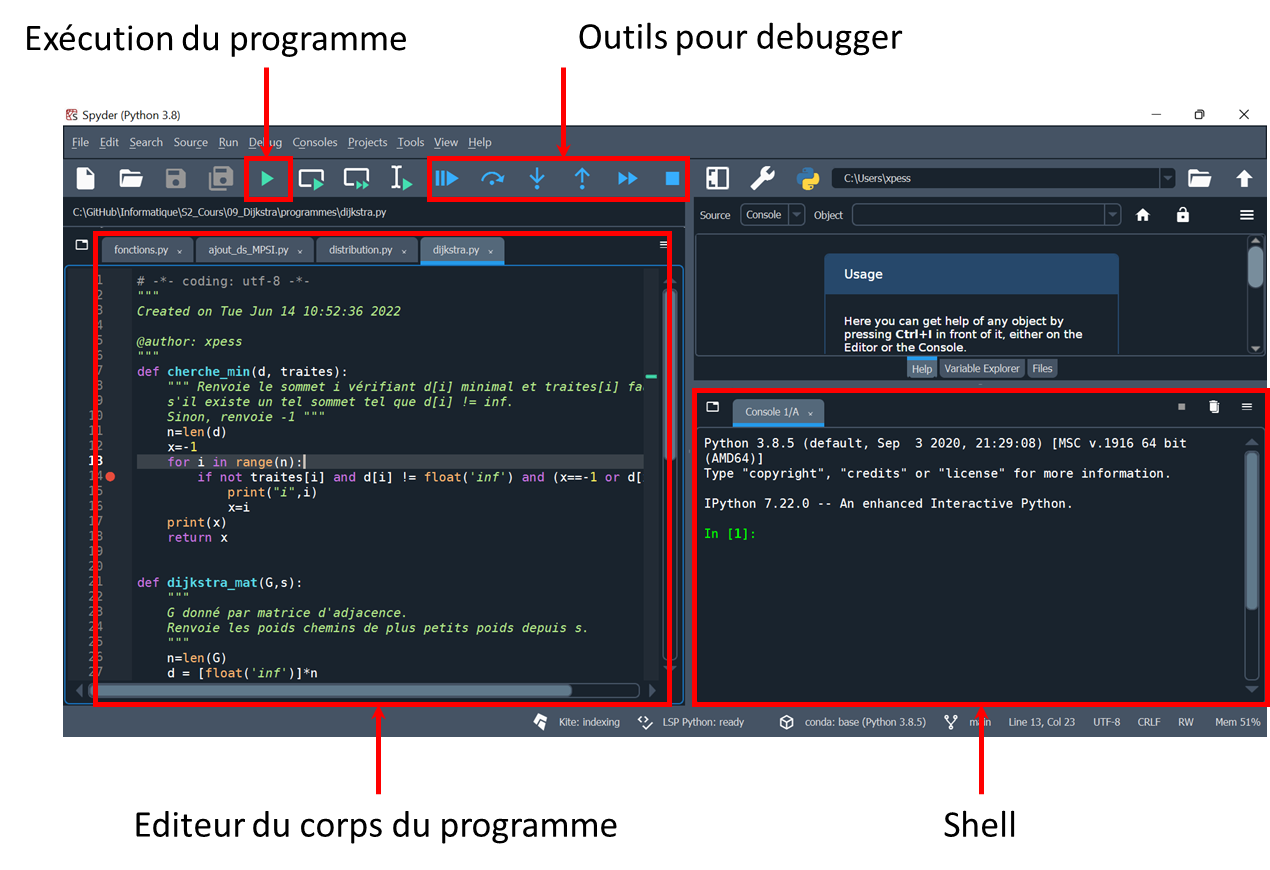
\includegraphics[width=12cm]{Spyder.png}
%\end{center}
\end{figure}

\section{Variables, Types}

\subsection{Quelques définitions}
\begin{defi}{Valeurs}
Les valeurs désignent les données manipulées par un algorithme ou une fonction. Une valeur 
peut ainsi être  : un nombre, un caractère, une chaîne de caractères, une valeur de vérité 
(\texttt{Vrai} ou \texttt{Faux}) \textit{etc}.

En Python, comme dans la plupart des langages de programmation, ces valeurs sont \textbf{typées} selon l'objet qu'elles représentent : il y a ainsi des valeurs de \textbf{type} entier, flottant, chaîne de caractères, booléens ...   Leur représentation en mémoire varie beaucoup d'un langage à l'autre, mais ce sont souvent les mêmes objets que l'on 
cherche à traduire.
\end{defi}

\begin{defi}{Expression }
Une expression est une suite de caractères faisant intervenir des valeurs et des 
opérations, afin d'obtenir une nouvelle valeur. Pour calculer cette nouvelle valeur,
la machine doit {évaluer} l'expression. Voici des exemples d'expressions : \texttt{42 , 1+4 , 
1.2 / 3.0 , x+3}.

\end{defi}


%\begin{xxpyconsole}%~\\ \vspace{-.5cm}
En Python, pour évaluer une expression, il suffit de la saisir dans un interpréteur (consoles), qui
calcule et affiche alors la valeur qu'il a calculée.
\begin{lstlisting}
>>> 42
	42
>>> 1+4
	5
\end{lstlisting}
%\end{xxpyconsole}



\begin{defi}{Variable}
Une \textbf{variable} désigne une zone mémoire de l'ordinateur dans la RAM.
Il s'agit d'un endroit où l'on peut \textbf{stocker} une valeur, y \textbf{accéder} et 
\textbf{changer} cette valeur.

Pour faire référence à une variable, on utilise un nom de variable, en général composé d'une ou 
plusieurs lettres. Dans la mesure du possible, on choisit un nom explicite, ce qui permet une 
meilleure lecture du programme.
\end{defi}





\subsection{Types simples}

En programmation, associer un type à une valeur permet :
\begin{itemize}
\item de classer les valeurs en catégories similaires. Par exemple, tous les
entiers (type int), tous les flottants (type float)...
\item de contrôler quelles opérations sont faisables sur ces valeurs : par
exemple, tout entier (type int) pourra être utilisé dans une soustraction, ..., alors 
qu'une chaîne ne le pourra pas. Il sera également impossible d'additioner un entier et un booléen. 
                                     
\end{itemize}

Une expression n'a a priori pas de type, car le type de la valeur qu'elle renvoie dépend des types 
des sous-expressions. Ainsi \texttt{a+b} sera un entier (resp. un flottant, une chaîne) si 
\texttt{a} et \texttt{b} le sont, mais sera un flottant si \texttt{a} est un entier et \texttt{b} 
un flottant.


%\begin{xxpyconsole}%~\\ \vspace{-.5cm}
Pour afficher le type d'une valeur ou d'une expression après l'avoir évaluée, on utilise 
\texttt{type}.
\begin{lstlisting}
>>> type(42)
	int
>>> type(1.2/3.0)
	float
\end{lstlisting}
%Le mot qui suit \texttt{class} indique le type de la valeur, entier (\texttt{int} en anglais) pour 
%la première et flottant (\texttt{float} en anglais) pour la seconde. Le mot \texttt{class} fait 
%référence au fait que Python, est un langage {orienté objet}, ce que nous ignorerons pour 
%l'instant.\\
%\end{xxpyconsole}





\subsubsection{Entiers}
\begin{defi}{Entiers}
Ce type est noté \texttt{int} en Python .\\
\begin{itemize}
\item \textbf{Constantes :} ce sont les entiers relatifs écrits en base 10. Ils ne sont pas 
bornés en Python .
\item \textbf{Opérateurs :}
\begin{enumerate}
 \item $+$ : addition usuelle;
 \item $-$ : soustraction usuelle (\texttt{15-9} renvoie \texttt{6}), mais aussi opposé (\texttt{-4});
\item  $//$ : {division entière} : \texttt{a//b} correspond au quotient de la 
division euclidienne de \texttt{a} par \textbf{b} si \texttt{b} est strictement positif 
(\texttt{256 // 3} renvoie \texttt{85} car $256 = 85*3 + 1$). Mais si \texttt{b} est strictement 
négatif, alors \texttt{a//b} renvoie ce quotient moins 1 ($15 = (-4)\times(-4)-1=(-4)\times(-3)+3$, 
le quotient de la division euclidienne de 15 par $-4$ est $-3$, mais \texttt{15//-4} renvoie 
\texttt{-4}). Cette division n'est pas définie si \texttt{b} est nul;
\item $\%$ : {modulo} : même remarque que dans le point précédent, relativement au reste de la 
division euclidienne cette fois (\texttt{256 \% 3} renvoie 
\texttt{1}, \texttt{15\%-4} renvoie \texttt{-1}).
\item $**$ : exponentiation (\texttt{2\raisebox{0.3ex}{**}3} renvoie \texttt{8}).
\end{enumerate}
\end{itemize}
Les {règles de précédence}, autrement dit les règles de priorité entre opérations, sont 
similaires aux règles mathématiques usuelles.
\end{defi}
\subsubsection{Flottants}
\begin{defi}{Flottants}
Ce type est noté \texttt{float} en Python .
\begin{itemize}
\item  \textbf{Constantes :} ce sont les {nombres à virgule flottante}. Nous en
donnerons une définition précise dans un chapitre ultérieur : pour simplifier, disons pour 
l'instant que ce sont des nombres à virgule, avec un nombre borné de chiffres dans leur écriture.
\item \textbf{Opérateurs : }
\begin{enumerate}
 \item $+$ : addition usuelle;
 \item $-$ : soustraction usuelle, et aussi opposé.
\item  $/$ : division usuelle.
\item $**$ : exponentiation. %Remarquer la différence entre \texttt{2\raisebox{0.3ex}{**}100} et  \texttt{2.\raisebox{0.3ex}{**}100} ou \texttt{2\raisebox{0.3ex}{**}100.}.
\end{enumerate}
\end{itemize}
%\noindent\textbf{Avertissement :} ce qui précédé est valable en Python 3. Attention à l'opérateur 
%\texttt{/} en Python 2 !!!!
\end{defi}

\subsubsection{Booléens}


\begin{defi}{Expression -- Booléen}
%\footnote{Le mot {booléen} a été donné en hommage au mathématicien  britannique George Boole.} }}
Ce type est noté \texttt{bool} en Python.
\begin{itemize}
\item \textbf{Constantes :} il y en a deux : \texttt{True} et \texttt{False}.
\item \textbf{Opérateurs :}
\begin{enumerate}
 \item \texttt{not} : négation usuelle;
 \item \texttt{and} : conjonction usuelle;
 \item \texttt{or} : disjonction usuelle.
\end{enumerate}
\item \textbf{Opérateurs de comparaison :}
\begin{enumerate}
 \item \texttt{==} : test d'égalité : \texttt{2==3} renvoie \texttt{False}, \texttt{4==4} renvoie 
\texttt{True}. %Problème : \texttt{0.1+0.2==0.3} renvoie \texttt{False} ! Nous y reviendrons plus tard. Il ne faut pas confondre \texttt{==} avec \texttt{=}, symbole de l'{affectation}.
 \item \texttt{!=} : \texttt{a != b} est une écriture équivalente à \texttt{not (a == b)}.
 \item \texttt{<,>,<=,>=} : ce à quoi on s'attend.
\end{enumerate}
\end{itemize}
\end{defi}


\begin{exemple}
\texttt{True or False} renvoie \texttt{True}. \texttt{not(False or True) and True} renvoie \texttt{False}.
\end{exemple}

\begin{rem}
Python \ permet les chaînes de comparaisons : \texttt{1<2<3} renvoie
\texttt{True}, et \texttt{(1<2<-2) and (-5<2<6)} renvoie \texttt{False}.
\end{rem}

\subsection{Conversions \textit{-- Cast}}

Il est possible de convertir en entier en flottant avec la fonction \texttt{float}. La réciproque est possible dans une certaine 
mesure : \texttt{float(2)} renvoie \texttt{2.0}, \texttt{int(2.0)} renvoie \texttt{2}, mais \texttt{int(2.5)} renvoie \texttt{2} et 
\texttt{int(-3.5)} renvoie \texttt{-3}.

La fonction \texttt{int} appliquée à un nombre flottant procède donc à une troncature, ce n'est pas la fonction donnant la partie entière d'un nombre flottant (fonction \texttt{floor} du module \texttt{math}).

\subsection{Types composés}
\begin{defi}{}
On dit qu'une valeur est de type composé si elle est formée à partir de plusieurs autres 
valeurs de types plus simples. De nombreuses constructions sont définies sur tous les types 
composés.
\end{defi}

\subsubsection{$n$-uplets ou tuples}

\begin{defi}{Tuple}
Ce type est noté \texttt{tuple} en Python .
\begin{itemize}
\item \textbf{Construction et composantes :} les $n$-uplets généralisent les couples. Un couple s'écrira \texttt{(a,b)}, un triplet 
\texttt{(a,b,c)} ... etc. Il existe même des 1-uplets : il faut les écrire \texttt{(a,)}.¨\\%, et non  \texttt{(a)} : cette dernière écriture est équivalente à \texttt{a}, tout simplement.\\
Il n'est pas obligatoire que les éléments d'un tuple soient de même type. Par exemple, 
\texttt{(1,1.2,True)} est un triplet tout à fait valable.\\
On accède à la $k\ieme$ coordonnée d'un tuple \texttt{t} par la commande \texttt{t[k]}. Attention : 
\textbf{en Python , les coordonnées sont numérotées à partir de 0} ! On dit que $k$ est 
l'{indice} de \texttt{t[k]}. Ainsi, si \texttt{t = (1,2,3)}, \texttt{t[0]} vaut 1, 
\texttt{t[2]} vaut 3, et \texttt{t[3]} n'existe pas.\\
On dit que les tuples sont \textbf{immuables} ou \textbf{non mutables}: il n'est pas possible de changer un élément d'un 
tuple.
\item \textbf{Opérateurs :}
\begin{enumerate}
 \item $+$ : concaténation. \texttt{(1,2,3)+(1,4,5,6)} renvoie \texttt{(1,2,3,1,4,5,6)};
 \item \texttt{len} : {longueur} du tuple. \texttt{len(1,2,3)} renvoie \texttt{3};
 \item \texttt{in} : test d'appartenance. \texttt{3 in (1,2,3)} renvoie \texttt{True}, alors que 
\texttt{3 in (1,2,4,5)} renvoie \texttt{False};
\item le {slicing}, qui permet de construire des sous-tuples : \texttt{(5,2,6,7,8,9)[1:5]} 
renvoie \texttt{(2,6,7,8)} (attention à la borne de droite !).\\
\end{enumerate}
\end{itemize}
\end{defi}

\subsubsection{Chaînes de caractères}
\begin{defi}{Chaînes de caractères}
Ce type est noté \texttt{str} en Python , pour {string} en anglais.
\begin{itemize}
\item \textbf{Construction et composantes :} ce sont des suites finies de caractères, un caractère étant en python un caractère du clavier. On 
les note entre guillemets ou apostrophes : \texttt{``Ceci est un chaîne de caractères''} ou  
\texttt{'Ceci est une chaîne de caractères'}. La chaîne vide se note \texttt{``}\texttt{''} ou 
\texttt{''}. Un caractère est une chaîne de longueur 1.\\
On accède aux composantes d'une chaîne de la même manière que pour un tuple.
\item \textbf{Opérateurs :} ce sont les mêmes que pour les tuples.
\end{itemize}
\end{defi}
\subsection{Listes}
\begin{defi}{Listes}
Ce type est noté \texttt{list} en Python .

Comme les tuples, les {listes} sont des suites finies de valeurs arbitraires, mais cette fois 
ils sont \textbf{mutables} : on peut changer la valeur d'une composante d'une liste.\\
Les listes s'écrivent entre crochets. On change la valeur de la $k\ieme$ composante d'une liste 
\texttt{L} grâce à la commande \texttt{L[k] = n}, où \texttt{n} est la nouvelle valeur. Ainsi :
\begin{lstlisting}
L = [1,2,3] 
L[0] = 4  
L 
\end{lstlisting}

Les autres opérateurs sont les mêmes que pour les tuples et les chaînes. Nous reviendrons plus tard sur les listes.
\end{defi}

\subsection{Conversions}

On peut convertir des types simples en chaînes avec la fonction \texttt{str} : \texttt{str(2.3)} 
renvoie \texttt{'2.3'}.\\
À l'inverse, \texttt{int, float} et \texttt{bool} permettent de faire l'inverse quand cela est 
cohérent : \textbf{bool('True')} renvoie \texttt{True}, mais \texttt{int('2.3')} renvoie une 
erreur.\\

Il est également possible de passer d'un type composé à un autre grâce aux fonctions \texttt{str}, 
\texttt{tuple} et \texttt{list} : \texttt{str((1,'a',[1,2]))} renvoie \texttt{''(1,'a',[1,2])''}, 
\texttt{tuple([1,2,3] )} renvoie \texttt{(1,2,3)} et \texttt{list('Coucou ?')} renvoie 
\texttt{['C', 'o', 'u', 'c', 'o', 'u', ' ', '?']}.

\subsection{Affectation}

\begin{defi}{Affectation}
Quand on stocke une valeur \texttt{d} dans une variable \texttt{var}, on dit que l'on 
\textbf{affecte} \texttt{d} à la variable \texttt{var}. La valeur
\texttt{d} est encore appelée \textbf{la donnée}.
\end{defi}

En Python , cette affectation est faite avec la commande \texttt{=}, comme suit.  

\begin{lstlisting}
>>> var  = 1
\end{lstlisting}


Les variables (et donc l'affectation) sont incontournables : si vous ne stockez pas une donnée 
(résultat par exemple d'un calcul), vous ne pourrez pas la réutiliser, ni la modifier.

%\begin{xxpyconsole}~\\ \vspace{-.5cm}%\begin{exemple}~
\begin{lstlisting}
>>> x = 42                 # x prend la valeur 42.
>>> x = x + 2	         # on additionne à la donnée stockée dans x le nombre 2 et on 
                 # stocke le résultat de nouveau dans x 
>>> x                  # on accède à la valeur qui est mémorisée dans x.
	44
\end{lstlisting}
%\end{xxpyconsole}
%\end{exemple}

Dans la variable affectée, la nouvelle donnée \og écrase\fg\ la donnée précédente : on perd son 
ancienne valeur.

Dans un programme Python, on utilisera l'instruction \texttt{print(x)}
pour afficher dans la console la valeur de la variable \texttt{x}.

Il est également possible d'affecter des valeurs à plusieurs variables en une fois, en utilisant 
des tuples. Ainsi : \texttt{a,b = (1,2)} affecte la valeur 1 à \texttt{a} et la valeur 2 à 
\texttt{b}.


\begin{rem}
En Python, le \textbf{typage} des variables est \textbf{dynamique}. Cela signifie que lorsqu'on affecte une valeur à une variable, Python reconnaît automatiquement le type de la valeur. Ce n'est pas le cas de tous les langages de programmation.
%Par exemple, le \texttt{C} n'est pas typé dynamiquement. Il faut alors déclarer une variable avec un type, puis affecter la valeur. 

\end{rem}
\subsubsection*{Notion d'adressage}

En Python, le passage des variables se fait par \textbf{référence}. C'est-à-dire que lorsqu'on manipule une variable (qu'on l'envoie à une fonction par exemple), on ne donne pas comme argument la valeur de la fonction, mais son adresse mémoire. Pour les types non mutables (entiers, flottants, chaîne de caractères, tuples), le passage par référence ne pose pas de problèmes. Pour les types mutables (listes), le passage par référence peut conduire à des résultats <<~inattendus~>> notamment lors de la copie de listes. 


%\begin{xxpyconsole}~\\ \vspace{-.5cm}
\begin{multicols}{2}
\begin{lstlisting}
>>> a=2
>>> print(a)
	2
>>> a=3
>>> print(a)
	3
>>> a=[1,2]
\end{lstlisting}

\begin{lstlisting}
>>> print(a)
	[1,2]
>>> b=a
>>> a[0]=2
>>> print(a,b)
	[2,2] [2,2]
\end{lstlisting}
\end{multicols}
Ici l'affectation \texttt{b=a} ne crée pas une nouvelle liste \texttt{b}. On crée juste une nouvelle variable \texttt{b} qui a la même adresse mémoire que \texttt{a}. Ainsi en modifiant \texttt{a}, on modifie \texttt{b}. 
%\end{xxpyconsole}



%%%%%%%%%%%%%%%%%%%%%%%%%%%




\section{Fonctions}
\subsection{Objectif : modularité des programmes}

Pour répondre à un problème donné, il est souvent nécessaire d'enchaîner plusieurs voire un nombre 
important d'instructions. Pour améliorer la lisibilité d'un programme et aussi pour pouvoir réutiliser 
ces instructions classiques (dans le même programme ou dans un autre),
on privilégie les programmes simples (ou sous-programmes) appelés \textbf{fonctions}.

Dans chaque langage, il y a déjà un nombre incalculable de fonctions déjà construites (en Python, 
par exemple, \texttt{print}) mais on s'aperçoit très vite que l'on a besoin de créer ses propres 
fonctions.


%\subsection{\'Ecriture en langage naturel}
%
%\fbox{\begin{minipage}{15cm}
%
%On appelle \texttt{DefFonction} l'opération qui consiste à définir une nouvelle fonction nommée 
%\textbf{nom-de-la-fonction} présentée comme suit : 
%\begin{center}
%\texttt{DefFonction} \begin{tabular}{|l}
%					\textbf{nom\_ de\_la\_fonction}(\textit{paramètres})\\
% \hspace{5ex} \og commentaire expliquant la fonction \fg\\
%\hspace{5ex}	bloc d'instructions\\
%\hspace{5ex}	sortie du résultat\\
%					\textbf{fin}
%					\end{tabular}
%\end{center}
%\end{minipage}}
%
%\vspace{0.5cm}
%\begin{exemple}
%On veut convertir en secondes une durée donnée en heures, minutes et secondes : 
%
%\texttt{DefFonction} 
%\begin{tabular}{|l}
%				\textbf{conversion}(h,m,s)\\
%\hspace{5ex}  \og convertit en secondes une durée donnée en heures,  minutes et secondes \fg\\
%\hspace{5ex} $t \leftarrow 3600*h+60*m+s$\\
%\hspace{5ex} Renvoyer t\\
%				  \textbf{fin}
%				  \end{tabular}
%
%\vspace{2ex}									
%\textbf{Une fois définie, pour l'utiliser, on écrit son nom suivi, entre parenthèses, des 
%paramètres.} 
%
%\vspace{0.2cm}
%Pour convertir 2h35mn45s, on écrit \textbf{conversion}(2,35,45) (réponse : 9345).

%\end{exemple}

\begin{rem}

\begin{itemize}
	\item Pour bien se faire comprendre, il est important de choisir un nom de fonction 
explicite. 
Il faut aussi mettre des commentaires pour expliquer ce que fait la fonction.
	\item Il est nécessaire de bien cibler les paramètres dont on a besoin 
c'est-à-dire les données nécessaires à l'exécution de la fonction.
	\item Il faut repérer ce que renvoie la fonction : rien (exemple : un simple affichage ou 
la modification d'un fichier...), un nombre entier, 
un flottant, une liste...
%
%Reprenons l'exemple de la conversion 
%
%\begin{description}
% \item[1er cas.] 
%\texttt{DefFonction} 
%\begin{tabular}{|l}
%				\textbf{conversion}(h,m,s)\\
% \hspace{5ex}  \og convertit en secondes une durée donnée en heures,  minutes et secondes \fg\\
%	\hspace{5ex} $t \leftarrow 3600*h+60*m+s$\\
%	\hspace{5ex} Renvoyer t\\
%				  \textbf{fin}
%				  \end{tabular}
%
%Si on écrit \texttt{rep}=\textbf{conversion}(h,m,s), on trouvera dans \texttt{rep} un nombre entier.
%
%\item[2ème cas.] 
%\
%
%\texttt{DefFonction} 
%\begin{tabular}{|l}
%				\textbf{conversion}(h,m,s)\\
% \hspace{5ex}  \og convertit en secondes une durée donnée en heures, minutes et secondes \fg\\
% \hspace{5ex} $t \leftarrow 3600*h+60*m+s$\\
% \hspace{5ex} Afficher t\\
%				  \textbf{fin}
%				  \end{tabular}
%
%Si on écrit \texttt{rep}=\textbf{conversion}(h,m,s), on  ne trouvera rien dans \texttt{rep} mais la 
%valeur s'affichera à l'écran.
%\end{description}

	\item Enfin, il faut toujours tester sa fonction sur un ensemble significatif de valeurs 
pour repérer d'éventuelles erreurs ou manquements.
\end{itemize}
\end{rem} 

\subsection{\'Ecriture en Python }

\begin{lstlisting}
def nom_de_la_fonction(parametres):
     """ commentaire expliquant la fonction """
     #bloc d'instructions
     return(resultat)
\end{lstlisting}

\begin{rem}
En Python , l'indentation est {signifiante} : après le mot-clé \texttt{def}, chaque 
ligne indentée fait partie de la fonction. La première ligne non indentée rencontrée marque la 
fin de la fonction : cette ligne ne fait plus partie de la fonction, mais celles qui précéde en 
font partie. Il est donc {impératif} d'indenter quand il le faut, et seulement 
quand il le faut.% On rencontrera ce phénomène constamment en Python .
\end{rem}

\subsubsection*{Annotations des fonctions}

Afin de préciser à l'utilisateur ou au lecteur de votre programmes quels sont les types d'arguments ou le type retourné par la fonction, il est possible d'utiliser des annotations. Celles-ci ont un rôle uniquement documentaire.
\begin{lstlisting}
def foo(par: int) -> float :   # Ces annotations indiquent que la fonction prend 
                                # comme un argument un entier 
                                # et renvoie un float.
     """ commentaire expliquant la fonction """
     #bloc d'instructions
     return(2.*par)
\end{lstlisting}

\section{Structures algorithmiques}
\subsection{L'instruction conditionnelle}

\subsubsection{Algorithme}

Quand on veut écrire un programme, on souhaite établir des connections logiques
entre les instructions. 
Ainsi, l'instruction conditionnelle a pour objet
d'intervenir dans le choix de l'instruction suivante en fonction d'une expression booléenne qu'on 
désignera par \textbf{condition} : 

%\vspace{1cm}
\begin{center}
\fbox{\begin{minipage}{12cm}

\begin{center}
\begin{tabular}{|l}
\textbf{Si} condition\\
\hspace{0.7cm}
\begin{tabular}{l}
\textbf{alors } bloc d'instructions 1\\
\textbf{sinon} bloc d'instructions 2\\
\end{tabular}\\
\textbf{Fin-du-Si}
\end{tabular}
\end{center}



\begin{center}
signifie que 
\end{center}

\begin{itemize}
\item \textbf{Si} la condition est vérifiée (expression booléenne=\texttt{True}) 

\textbf{alors} le programme exécute les instructions du bloc 1;

\item \textbf{si} la condition n'est pas vérifiée (expression booléenne=\texttt{False})

\textbf{alors }le programme exécute les instructions du bloc 2.
\end{itemize}
\end{minipage}}

\end{center}
%\newpage


\subsubsection{Syntaxe en Python}

%\begin{lstlisting}
\begin{lstlisting}
if condition : 
	bloc d instructions 1
else :
	bloc d instructions 2
\end{lstlisting}


 \begin{itemize}
 \item \textbf{Si} et \textbf{Sinon} se traduisent par \texttt{if} et \texttt{else}. 
 
 \item \textbf{Alors} se traduit par \og \textbf{:} \fg\ en bout de ligne et une indentation de toutes les 
lignes du bloc 1.
 
 \item \textbf{Fin-du-Si} se traduit par un retour à la ligne sans indentation. 
 
 \end{itemize}

 
\subsubsection{Exemple}

On veut tester si un nombre $x$ est proche de 3 à $10^{-4}$ près. On peut alors écrire la fonction suivante. 

\begin{lstlisting}
def est_proche(x):
    """x est proche de 3 à 10**-4 près ?"""
    distance = abs(x-3)
    if distance <= 10**(-4) : 
        return True 
    else : 
        return False
\end{lstlisting}



\begin{rem} 
La partie \textbf{sinon} est optionnelle. Sans elle, si la condition n'est pas vérifiée, alors la 
machine n'exécute rien.
\end{rem}

\begin{rem}
  On pouvait très bien remplacer cette boucle conditionnelle avec un usage astucieux des booléens, comme suit.
\begin{lstlisting}
def est_proche(x):
    """x est proche de 3 à 10**-4 près ?"""
    distance = abs(x-3)
    return distance <= 10**(-4)
\end{lstlisting}
La fonction est alors plus concise, mais plus difficilement lisible. 
\end{rem}


\subsubsection{\`A propos des conditions}

L'expression booléenne derrière le \textbf{si} joue le rôle de test. Pour exprimer cette condition, 
on a besoin des \textbf{opérateurs de comparaison} (inférieur strict, supérieur strict, inférieur ou 
égal, supérieur ou égal, égal à, différent de) et des \textbf{connecteurs logiques}
(non, et, ou).

%\begin{exs}

\begin{multicols}{2}
\begin{itemize}

\item Calcul du carré d'un nombre positif. 

\begin{lstlisting}
>>> x=4
>>> if x >= 0 : 
        car = x**2

>>> car 
	16
\end{lstlisting}

\vfill\null
\columnbreak 


\end{itemize}
\end{multicols}
\begin{itemize}

\item Condition avec un \og et \fg{}. 

\begin{lstlisting}
x = 0.5 
if x >= -1 and x <= 1 :
    print("Il existe un angle theta tel que x = cos(theta).") 

\end{lstlisting}
 \end{itemize}

% \end{exs}




%\newpage
\subsubsection{Imbrication de plusieurs conditions}

On peut se trouver face à un problème qui se scinde en plus de deux cas (par exemple, dans le cas 
des équations du second degré, on teste si le discriminant est strictement positif, nul ou 
strictement négatif).
Dans ce cas, voici comment procéder.
%
%\begin{center}
%
%
%\fbox{\begin{minipage}{15cm}
%
%\begin{center}
%\begin{tabular}{|l}
%\textbf{Si} condition 1\\
%\hspace{0.7cm}
%\begin{tabular}{l}
%\textbf{alors} bloc d'instructions 1\\
%\textbf{sinon si} condition 2\\
%\hspace{0.7cm}
%\begin{tabular}{l}
%\hspace{7ex}\textbf{alors} bloc d'instructions 2\\
%\hspace{7ex}\textbf{sinon si} condition 3\\
%\hspace{14ex}\textbf{alors} bloc d'instructions 3\\
%\ldots\\
%\hspace{14ex}\textbf{sinon} bloc final
%\end{tabular}\\
%\end{tabular}\\
%\textbf{Fin-du-Si}
%\end{tabular}
%\end{center}
%
%\begin{center}
%signifie que 
%\end{center}
%
%\begin{itemize}
%\item \textbf{Si} la condition 1 est vérifiée (expression booléenne=\textit{True}) 
%
%\textbf{alors} le programme exécute les instructions du bloc 1.
%
%\item \textbf{Si} la condition 1 n'est pas vérifiée (expression booléenne=\textit{False}) mais que 
%la condition 2 est vérifiée
%
%\textbf{alors} le programme exécute les instructions du bloc 2.
%
%\item \textbf{Si} les conditions 1 et 2 ne sont pas vérifiées  mais que la condition 3 est vérifiée
%
%\textbf{alors} le programme exécute les instructions du bloc 3...
%
%\item \textbf{Si} aucune condition n'est vérifiée
%
%\textbf{alors} le programme exécute les instructions du bloc final.
%\end{itemize}
%\end{minipage}}
%
%\end{center}
%
%\vspace{0.5cm}
%\begin{rem}\label{rem-filtre}
%\begin{itemize}
%\item Si la \texttt{condition 1} est vérifiée, le programme ne se préoccupe pas des conditions 
%suivantes.
%\item Chaque \textbf{sinon si} agit comme un \textbf{filtre}. L'ordre de ces filtres est important. 
%Ainsi, les séquences d'instructions :\\
%
%\begin{tabular}{|l}
% $x \leftarrow$ 3 \\
%\textbf{Si} $x >$ 6\\
%\hspace{0.7cm}
%\begin{tabular}{l}
%\textbf{alors} renvoyer $x + 2$\\
%\textbf{sinon si} $x > 4$\\
%\hspace{0.7cm}
%\begin{tabular}{l}
%\hspace{7ex}\textbf{alors} renvoyer $x + 4$\\
%\hspace{7ex}\textbf{sinon si}$ x > 2$\\
%\hspace{14ex}\textbf{alors} renvoyer $x + 6$\\
%\hspace{14ex}\textbf{sinon} renvoyer $x$
%\end{tabular}\\
%\end{tabular}\\
%\textbf{Fin-du-Si}
%\end{tabular}\\
%
%et \\
%
%\begin{tabular}{|l}
% $x \leftarrow 3$\\
%\textbf{Si} $x > 6$\\
%\hspace{0.7cm}
%\begin{tabular}{l}
%\textbf{alors} renvoyer $x + 2$\\
%\textbf{sinon si} $x > 2$\\
%\hspace{0.7cm}
%\begin{tabular}{l}
%\hspace{7ex}\textbf{alors} renvoyer $x + 6$\\
%\hspace{7ex}\textbf{sinon si} $x > 4$\\
%\hspace{14ex}\textbf{alors} renvoyer $x + 4$\\
%\hspace{14ex}\textbf{sinon} renvoyer $x$
%\end{tabular}\\
%\end{tabular}\\
%\textbf{Fin-du-Si}
%\end{tabular}\\
%
%
%ne renvoient pas la même chose.
%
%\end{itemize}
%\end{rem}

%\subsubsection{Syntaxe en Python}

\begin{lstlisting}
 if condition 1 :
	bloc d instructions 1
 elif condition 2 :
	bloc d instructions 2
 elif condition 3 :
	bloc d instructions 3
.
.
.
 else :
	bloc final
\end{lstlisting}

\begin{itemize}
 \item \textbf{Sinon si} se traduit par \texttt{elif}. 
\end{itemize}

%\begin{exo}
\begin{exemple}
Écrire les deux séquences d'instructions de la remarque \textbf{\ref{rem-filtre}} en Python, et 
constater que l'on obtient bien deux résultats différents.
\end{exemple}
%\end{exo}

%\begin{ex}
Voici une fonction qui calcule le maximum de trois entiers \texttt{a, b, c} :
\begin{lstlisting}
def max3 (a, b, c) :
    """ renvoie le maximum de a, b ,c.
    précondition : a, ,b et c sont 3 entiers """
    if a <= c and b <= c :
        return c
    elif a <= b and c < b :
        return b
    else :
        return a
\end{lstlisting}

%\end{ex} 


\subsection{Boucles définies}

%\subsubsection{Un programme très simple}
%
%Écrivons un programme pour saluer la classe (disons les 8 premiers
%élèves) :
%\begin{lstlisting}
%print('Bonjour Baptiste')
%print('Bonjour Lisa')
%print('Bonjour Pierrick')
%print('Bonjour Louise-Eugénie')
%print('Bonjour Qasim')
%print('Bonjour Lorenzo')
%print('Bonjour Arthur')
%print('Bonjour Ylies')
%\end{lstlisting}
%
%Mais combien de travail faut-il faire si :
%
%\begin{itemize}
%\item on veut dire bonsoir et non bonjour?
%\item on veut dire «Baptiste, comment vas-tu? \textit{etc.}» et non
%  «Bonjour Baptiste, \textit{etc.}» ?
%\end{itemize}
%
%Et s'il y a 500 élèves ?
%
%
%\subsection{Le principe DRY}
%
%«\textbf{D}on't \textbf{R}epeat \textbf{Y}ourself» est une philosophie en programmation 
%informatique consistant à éviter la redondance de code au travers de l'ensemble d'une application 
%afin de faciliter la maintenance, le test, le débogage et les évolutions de cette dernière.\\
%La philosophie DRY est explicitée par la phrase suivante :\\
%  \textit{«Dans un système, toute connaissance doit avoir une représentation
%   unique, non-ambiguë, faisant autorité ».}
%
%Ici le programme devrait:
%\begin{itemize}
%\item définir la liste des prénoms auxquels dire bonjour;
%\item dire qu'on veut effectuer un même traitement sur tous les prénoms;
%\item dire que ce traitement consiste à afficher «Bonjour» suivi du prénom.
%\end{itemize}
%
%
%Nous avons déjà vu comment définir une liste :
%
%\begin{lstlisting}
%prenoms = [ 'Baptiste', 'Lisa', 'Pierrick',\
%'Louise-Eugénie', 'Qâsim', 'Lorenzo', 'Arthur', 'Ylies' ]
%\end{lstlisting}
%
%Il faut maintenant s'occuper des deux points suivants : définir le traitement à effectuer sur 
%chacun de ces 
%prénoms, et l'\textbf{itérer}. Pour cela nous allons utiliser une \textbf{boucle itérative 
%définie}, autrement dit nous allons \textbf{répéter} l'application d'une même séquences
%d'instructions 
%sur une liste \textbf{définie à l'avance}.


\fbox{\begin{minipage}{12cm}

\begin{center}
\begin{tabular}{|l}
\textbf{Pour} variable \textbf{dans} liste \textbf{répeter}\\
\hspace{0.7cm}
\begin{tabular}{l}
bloc d'instructions b\\
\end{tabular}\\
\textbf{Fin-de-la-boucle}
\end{tabular}
\end{center}



\begin{center}
signifie que 
\end{center}

\textbf{pour} chaque élément de la liste \texttt{liste},

le programme exécute les instructions du bloc b.

\end{minipage}}


\subsubsection{Syntaxe en Python}

\begin{lstlisting}
for variable in liste :
    instructions
\end{lstlisting}

Ici encore, la ligne contenant le mot-clé \textbf{for} doit se finir par un \og \textbf{:} \fg\ et les 
instructions du bloc doivent être indentées. La fin de la boucle est marquée par un retour à la 
ligne non indenté.\\
%
%Maintenant que la liste \texttt{prenoms} est définie, dire bonjour à nos huit élèves s'écrit ainsi :
%
%
%\begin{lstlisting}
%for x in prenoms:
%    print('Bonjour ' + x)
%\end{lstlisting}
%


%\end{enumerate}

\subsubsection{Les intervalles d'entiers en Python}

Pour répondre à la première question, il suffit de remarquer que les entiers de 0 à 19 par exemple, 
sont en fait les éléments d'une liste : \texttt{[0, 1, 2, $\cdots$ , 19]}. En Python, cette liste 
s'écrit de la manière suivante : \texttt{range(20)}.\\
Précisément, si $a$ et $b$ sont deux entiers, \texttt{range(a,b)} contient les éléments de 
l'intervalle semi-ouvert $\ii{a,b}$, dans l'ordre croissant. Avec un seul argument, 
\texttt{range(b)} signifie \texttt{range(0,b)}.\\

\textbf{
Redisons-le, car c'est un fait important en Python : \texttt{range(a,b)} est intervalle 
\textbf{fermé} à gauche, \textbf{ouvert} à
droite}\footnote{Voir \textit{Why numbering should start at zero}, E. W. Dijkstra,
  EWD831. Disponible en ligne.}.\\
  
Avec \texttt{range}, nous pouvons maintenant itérer sur une liste d'entiers :

\begin{lstlisting}
x = 5
for k in range(20):
    x = 2 * x - k - 3
  
print(x)
#  Résultat obtenu : 1048600.
\end{lstlisting}

%
%\begin{rem}
%Mais est-ce bien $u_{20}$ ? Pour cela on pourra montrer par récurrence que $x=u_k$ à l'entrée de la boucle et $x=u_{k+1}$ à la sortie de la boucle. C'est la notion \textbf{d'invariant de boucle} que l'on détaillera dans un chapitre ultérieur.
%\end{rem}

%\subsection{Les invariants de boucle}
%
%Un \textbf{invariant de boucle} est une proposition vérifiée à chaque tour d'une boucle. Plus 
%précisément, on distingue les invariants d'\textbf{entrée de boucle} et ceux de \textbf{sortie de 
%boucle}. C'est en fait une proposition de récurrence, qui doit être vrai au début de la première 
%boucle, puis se propager de tour de boucle en tour de boucle, jusqu'au dernier.\\
%Les invariants de boucles ont essentiellement deux intérêts :
%\begin{enumerate}
% \item \textbf{Démontrer} l'algorithme, grâce au principe de récurrence ;
% \item Répondre à notre question précédente : où commencer et où finir une boucle ?
%\end{enumerate}
%
%Il est \textbf{fortement conseillé} de toujours indiquer les invariants de boucle en commentaire 
%dans vos algorithmes.\\ 
%
%Par exemple :
%
%
%\begin{lstlisting}
%x = 5			# x = u_0 (initialisation)
%for k in range(20): 	
%    # x = u_k (invariant en entrée de boucle)
%    x = 2 * x - k - 3	
%    # x = u_{k+1} (invariant en sortie de boucle)	
%# après la boucle for, k vaut 19, et x vaut donc u_{20}.
%\end{lstlisting}
%  


%\subsection{Un exemple : test de primalité} 
%
%  On veut tester si un entier \texttt{n} est premier:
%\begin{lstlisting}
%def est_premier(n):
%    """ Renvoie True si n est premier, False sinon
%        Préconditon : n est un entier."""
%    b = True
%    for d in range(2,n):
%        # b => n non divisible par 2, 3, ..., d-1.
%        if n % d == 0:
%            b = False
%    # b <=> n premier
%    return b
%\end{lstlisting}
%
%Remarque: les derniers tours de boucle sont inutiles dès que la
%variable \texttt{b} a été mise à \texttt{False}. Les éxécuter tout de même est une perte de temps. Il 
%existe plusieurs possibilités pour améliorer cela~:
%
%L'instruction \texttt{break} :
%\begin{lstlisting}
%def est_premier(n):
%    """ Renvoie True si n est premier, False sinon
%        Préconditon : n est un entier."""
%    b = True
%    for d in range(2,n):
%        # b => n pas divisible par 2, 3, ..., d-1.
%        if n % d == 0:
%            b = False
%            break
%    # b <=> n est premier
%    return b
%\end{lstlisting}
%
%L'utilisation d'un \texttt{return} en milieu de boucle, à favoriser en Python{} pour 
%une question de style et d'élégance~:
%
%\begin{lstlisting}
%def est_premier(n):
%    """ Renvoie True si n est premier, False sinon
%        Préconditon : n est un entier."""
%    for d in range(2,n):
%        # n n'est pas divisible par 2, 3, ..., d-1.
%        if n % d == 0:
%            return False
%    return True
%\end{lstlisting}

\subsection{Boucles indéfinies ou conditionnelles}

\subsubsection{Algorithme}

On peut aussi être amené à répéter un bloc d'instructions sans savoir combien de fois on devra le 
répéter. 

%\begin{ex}
Disposant d'une suite croissante, non majorée, on cherche à trouver le plus petit entier $p$ 
tel que la valeur au rang $p$ dépasse 10000.
%\end{ex}

Dans ce cas, on utilise la boucle \textbf{Tant que} qui permet de répéter le bloc d'instructions 
tant qu'une certaine condition est vérifiée.


\vspace{1cm}


\fbox{\begin{minipage}{15cm}
\begin{center}
\begin{tabular}{|l}
\textbf{Tant que} condition\\
\hspace{0.7cm}
\begin{tabular}{l}
\textbf{faire } bloc d'instructions \\
\end{tabular}\\
\textbf{Fin-du-Tant-que}
\end{tabular}
\end{center}

\begin{center}
signifie que 
\end{center}

\begin{description}
\item[Tant que] la condition est vérifiée (expression booléenne=\textit{True}) 

\item[Faire]  le bloc d'instructions.
\end{description}
\end{minipage}}

\subsubsection{Syntaxe en Python}


\begin{lstlisting}
while condition :
    instructions
\end{lstlisting}



\vspace{0.5cm}
%\begin{ex}
\label{ex-suite}
Rechercher le premier entier $n$ tel que la somme des entiers de 1 à n dépasse 11.

\begin{lstlisting}
n = 1
s = 1
while s < 11 :
    n = n + 1
    s = s + n
    
n
# REPONSE  : n=5  (dans ce cas s=15)
\end{lstlisting}


%\end{ex}


%\begin{ex}
%\label{ex-syracuse} Conjecture de Syracuse :\\
%On note $f : \N^{*} \to \N^{*}$ l'application vérifiant, pour tout $n$ pair
%$f(n)=n/2$ et tout $n$ impair et $f(n)=3n+1$.
%
%On conjecture que pour tout entier $n$, il existe $k$ tel que
%$f^{k}(n)=1$.
%
%Voici un algorithme calculant, pour tout $n$ donné, le plus petit
%entier $k$ vérifiant $f^{k}(n) = 1$ :
%
%\begin{lstlisting}
%\begin{lstlisting}
%def f(n):
%    """Fonction de Syracuse.
%    Précondition : n est un entier strictement positif"""
%    if n % 2 == 0:
%        return n // 2
%    else:
%        return 3 * n + 1
%        
%def syracuse(n):
%    """Renvoie le premier entier k tel que  f\^k(n) = 0.
%    Précondition : n est un entier strictement positif"""
%    x = n
%    k = 0
%    while x != 1:
%        x = f(x)
%        k = k + 1
%    return k
%\end{lstlisting}
%%\end{lstlisting}
%
%%\end{ex}
%
%
%\begin{rem}
%\begin{itemize}
%\item Comme pour les boucles définies, nous sommes confrontés à un problème : comment démontrer un 
%algorithme reposant sur une boucle indéfinie ? Pour cela, nous utilisons encore les invariants de 
%boucle, afin de prouver qu'après la boucle, le résultat est bien celui voulu.
%\item Pour montrer que la boucle \textbf{while} va réellement se finir on utilisera un \textbf{variant} de boucle. Cette notion sera également détaillée dans un chapitre ultérieur. Dans un premier temps nous retiendrons que généralement il faudra s'assurer que la condition contenu dans la boucle \textbf{while} sera généralement une suite d'entiers strictement croissante ou décroissante.
%\end{itemize}
%\end{rem}
%Mais avant même cela, il y a un point épineux : la boucle \textbf{while} va-t-elle vraiment se 
%finir ? Il faut démontrer ce que l'on appelle la \textbf{terminaison} de l'algorithme. C'est là que 
%réside le danger des boucles \textbf{while} : si elles sont mal écrites, la condition de la boucle 
%ne devient jamais fausse, et la boucle est infinie.\\
%Pour montrer la terminaison d'un algorithme, on utilise cette fois un \textbf{variant} de boucle. 
%Il consiste à mettre en avant une variable dont la valeur est modifiée au cours des tours de 
%boucle, de telle sorte que cette modification finisse par rendre fausse la condition de la boucle.\\
%Donnons ces invariant et variant pour l'algorithme de l'exemple \textbf{\ref{ex-suite}} (nous ne 
%pouvons malheureusement pas le faire pour l'exemple \textbf{\ref{ex-syracuse}}, puisque comme son 
%nom l'indique, la conjecture de Syracuse n'a jamais été demontrée) :\\


%\begin{lstlisting}
%n = 1
%s = 1           # s = somme des i de 1 à n
%while s < 11 :  # invariant : s = somme des i de 1 à n
%    n = n + 1
%    s = s + n   # variant : s, qui est entier et strictement croissant
%\end{lstlisting}

%\begin{exo}
%Démontrer cet algorithme.
%\end{exo}


%\subsection{Exercices}
%
%\begin{exo}
% Calculer $2^9$ à l'aide d'une boucle itérative.
%\end{exo}
%
%
%\begin{exo}
% \'Ecrire un algorithme affichant la table de multiplication de 9.
%\end{exo}
%
%\begin{exo}
% Calculer $16!$ à l'aide d'une boucle itérative.
%\end{exo}
%
%\begin{exo}
% Calculer
%  \begin{equation*}
%    \sum_{k=0}^{15} \frac{1}{k!}
%  \end{equation*}
%\end{exo}
%
%\begin{exo}
% Écrire une fonction calculant le nombre de chiffres d'un entier écrit en base 10.
%\end{exo}
%
%\begin{exo}
% On considère la suite $u$ définie par
%\begin{equation*}
%  \forall n\in \N^{*}\quad u_{n} = \sum_{k=1}^{n} \frac{1}{\sqrt{k}}
%\end{equation*}
%
%Quel est la plus petite valeur $n$ pour laquelle $u_{n}\geq 1000$?
%\end{exo}
%
%\begin{exo}
% Écrire une fonction trouvant le plus petit nombre premier supérieur ou
%égal à un entier donné.
%\end{exo}
%
%\begin{exo}
% Écrire une fonction calculant le nombre de diviseurs d'un entier $n$ donné.
%\end{exo}
%
%%\begin{exo}
% Calculer $p_{5}/q_{5}$ où $p$ et $q$ sont définies par:
%  \begin{align*}
%    p_{0} &= 1\\
%    q_{0} &= 1\\
%    \forall n\in \N \quad p_{n+1} &= p_{n}^{2} + 2q_{n}^{2}\\
%    \forall n\in \N \quad q_{n+1} &= 2p_{n}q_{n}
%  \end{align*}
%\end{exo}
%
%\begin{exo}
%  %\exer{}
%\setcounter{numques}{0}

\question{Définir la fonction $f$ qui à $x$ associe $\left\{\begin{array}{rcl}
							     2 & \mathrm{si} & x \in [-4,-2]\\
							    -x & \mathrm{si} & x \in [-2,0]\\
							      0 & \mathrm{si} & x \in [0,4]\\
							      \end{array} \right.$
							      }
							      
\question{Ecrire une fonction calculant le produit des entiers impairs de 1 à $2n+1$.}

%\question{
\begin{enumerate}[label = \emph{\alph*)}]
  \item \'Ecrire une fonction \texttt{neg(b)} qui renvoie la négation du booléen \texttt{b} sans utiliser \texttt{not}.
  \item \'Ecrire une fonction \texttt{ou(a,b)} qui renvoie le ou logique des booléen \texttt{a} et \texttt{b} sans utiliser \texttt{not}, \texttt{or} ni \texttt{and}.
  \item \'Ecrire une fonction \texttt{et(a,b)} qui renvoie le et logique des booléen \texttt{a} et \texttt{b} sans utiliser \texttt{not}, \texttt{or} ni \texttt{and}.
\end{enumerate}%
%}
%\end{exo}
%
%\begin{exo}
%  \exer{}
\setcounter{numques}{0}

Écrire une fonction calculant le produit des entiers impairs de 1 à $2n+1$.
%\end{exo}
%
%\begin{exo}
%  \exer{}
\setcounter{numques}{0}

% \question
\begin{enumerate}[label = \emph{\alph*)}]
  \item \'Ecrire une fonction \texttt{neg(b)} qui renvoie la négation du booléen \texttt{b} sans utiliser \texttt{not}.
  \item \'Ecrire une fonction \texttt{ou(a,b)} qui renvoie le ou logique des booléen \texttt{a} et \texttt{b} sans utiliser \texttt{not}, \texttt{or} ni \texttt{and}.
  \item \'Ecrire une fonction \texttt{et(a,b)} qui renvoie le et logique des booléen \texttt{a} et \texttt{b} sans utiliser \texttt{not}, \texttt{or} ni \texttt{and}.
\end{enumerate}

%\end{exo}
%
%\begin{exo}
%  \exer{}
\setcounter{numques}{0}

% \question 
Indenter de deux manières différentes la suite d'expressions suivante de manière à ce qu'à son exécution, le programme affiche soit la liste de tous les éléments de $L$ inférieurs ou égaux à $m$, soit juste le dernier.
\begin{lstlisting}

from random import randrange
L = [randrange(100) for i in range(100)] # 100 valeurs entre 0 et 99.
m = 50
for x in L:
if x <= m:
p = x
print(p)
\end{lstlisting}


%\end{exo}
%
%
%\begin{exo}
%  \exer{}
\setcounter{numques}{0}

% \question 
Décrire ce que fait cette suite d'instructions. 
\begin{lstlisting}

from random import randrange
# Un entier entre 0 et 999
n = randrange(1000) 
# n+1 valeurs entre 0 et 99.
L = [randrange(100) for i in range(n+1)] 
p = 0
for x in L:
    if x <= 10:
        p = p + x**2
\end{lstlisting}

Et celle-ci ? 
\begin{lstlisting}

from random import randrange
# Un entier entre 0 et 999
n = randrange(1000) 
# n+1 valeurs entre 0 et 99.
L = [randrange(100) for i in range(n+1)] 
p = 0
for i in range(n+1):
    if L[i] <= 10:
        p = p + i**2
\end{lstlisting}


%\end{exo}
%
%
%\begin{exo}
%  \exer{}
\setcounter{numques}{0}

% \question 
\'Ecrire une suite d'instructions permettant de calculer la somme des racines carrées des cinquante premiers entiers naturels non nuls. 

%\end{exo}
%
%\begin{exo}
%  \exer{}
\setcounter{numques}{0}

% \question 
\'Ecrire la suite d'instructions suivantes dans un fichier, l'enregistrer puis l'exécuter (F5). \`A l'instant qui vous convient, presser Ctrl+C.
\begin{lstlisting}

a = 1
while a>0:
    a = a+1
\end{lstlisting}


%\end{exo}
%
%\begin{exo}
%  \exer{}
\setcounter{numques}{0}

% \question 
\question{Que fait la fonction suivante ? La corriger pour qu'elle coïncide avec le but annoncé.}

\begin{lstlisting}

def sqrt_int(n):
    """Renvoie la partie entière de la racine carrée de n"""
    s = 0
    while s**2 <= n:
        s = s+1
        s = s-1
    return s
\end{lstlisting}


%\end{exo}


\section{Tableaux et type \texttt{list} en \texttt{python}}

\subsection{Deux structures de données en informatique.}

Les données manipulées en informatique sont organisées, que ce soit dans la mémoire où dans la manière d'y accéder, de les manipuler. 
Une telle organisation porte le nom de \textbf{structure de données}, en voici deux grandes.  

\begin{defi}{}
  
  \textbf{Tableaux} --  
  Les données sont stockées dans des cases contiguës de la mémoire de l'ordinateur, chaque emplacement étant souvent indicé par un entier. 
    A priori, il n'est pas possible d'en rajouter autant que possible : cette place a été pré-allouée. 
    Pour accéder au contenu de l'emplacement numéro $k$, la machine a seulement besoin de connaître 
l'adresse de la première case mémoire et de la largeur de chaque case (faire un dessin). 
    L'accès en lecture et en écriture à une donnée (à partir du numéro de son emplacement) se fait donc en temps constant (on dit $\mathcal{O}(1)$).
    L'ajout d'une nouvelle donnée à un tableau peut alors être problématique !


  \textbf{Liste (chaînée)}  -- Les données ne sont pas stockées de manière organisée dans la mémoire, 
mais de chaque emplacement on pointe l'emplacement suivant. 
    Ainsi, l'accès (en lecture ou en écriture) ne se fait plus en temps constant, mais l'ajout d'une nouvelle donnée se fait simplement en temps constant. 
\end{defi}

\subsection{Et en \texttt{python}...}

Les objets de type \texttt{list} en Python sont des tableaux : c'est une 
dénomination fâcheuse car, partout ailleurs en informatique, le terme
\textbf{liste} désigne en fait une liste chaînée. Prenez donc
l'habitude de dire \og tableau\fg, ou \og liste Python \fg\ et non \og liste\fg\ quand vous parlez de cette
structure.

Cependant, il y a une raison à cette dénomination : ces tableaux en Python possèdent presque 
la propriété des listes, dans le sens où l'ajout d'un nouvel élément se fait en temps constant 
\textbf{amorti}. Cela signifie que la plupart de ces ajouts se font en temps constants car en fait 
Python a \og gardé des cellules en réserve\fg, mais parfois l'ajout d'un élément force la création 
d'un nouveau tableau avec plus de cellules de réserve, et la copie de l'ancien tableau dans le 
nouveau. Cette opération est coûteuse, mais elle 
est rare. En moyenne, chaque ajout à un coût constant.

On parle alors de \textbf{tableaux dynamiques}.

\begin{multicols}{2}
Pour créer un tableau on peut le donner en extension.

\begin{lstlisting}
t = [23, 41, 101]
t
\end{lstlisting}

On peut aussi le donner en compréhension.

\begin{lstlisting}
u = [k**2 for k in range(10)]
u
\end{lstlisting}
On peut alors accéder à ses éléments via leur indice.
\begin{lstlisting}
t[0]
u[1]
u[9]
\end{lstlisting}

Attention à utiliser un indice existant !
\begin{lstlisting}
>>> t[3]
\end{lstlisting}
%Traceback (most recent call last):
%  File "<stdin>", line 1, in <module>
%IndexError: list index out of range

Les indices appartiennent à $\ii{0,\texttt{len(t)}}$.
%\clearslide{}
Mais on peut aussi compter les éléments à partir de la fin, en utilisant des indices négatifs !
\begin{lstlisting}
t[-1] # dernier élément
t[-2] # avant-dernier
t[-3]
\end{lstlisting}

Attention, là aussi, à ne pas sortir du tableau !

\begin{lstlisting}
>>> t[-4]
Traceback (most recent call last):
  File "<stdin>", line 1, in <module>
IndexError: list index out of range
\end{lstlisting}

Enfin, il y a une liste Python particulière : la liste vide~\texttt{[]}.

\end{multicols}


\subsection{Opérations usuelles}

\subsubsection{Concaténation}
Concaténer deux tableaux revient à les mettre bout à bout, on l'effectue en Python avec 
l'opérateur \texttt{+}.
\begin{lstlisting}
t+u
u+t
\end{lstlisting}
Dans cette opération, les deux tableaux sont intégralement recopiés. 

\subsubsection{Quelques calculs}
La longueur se calcule avec la fonction \texttt{len}. Pour des listes Python de nombres, le maximum 
se calcule avec la fonction \texttt{max}, le minimum avec \texttt{min} et la somme des éléments de la 
liste avec \texttt{sum}.
\begin{lstlisting}
len(t)
max(t)
min(t)
sum(t)
\end{lstlisting}

On peut aussi tester l'appartenance d'un élément dans une liste Python avec \texttt{in}.

\begin{lstlisting}
42 in t
[] in [[]]
\end{lstlisting}

Enfin, on peut recopier plusieurs fois un \textbf{même} tableau avec l'opérateur \texttt{*}.

\begin{lstlisting}
4*t
t*4
\end{lstlisting}




\subsubsection{Un peu de méthodes}
Python est un langage \textbf{orienté objet} : en \texttt{python}, tout est un \textbf{objet}, et ces objets 
sont regroupées en \textbf{classes}. Une \textbf{méthode} est une fonction qui s'applique aux objets 
d'une classe particulière. Si \texttt{method} est une méthode de la classe \texttt{c}, et si 
\texttt{a} est un objet de cette classe, alors on applique \texttt{method} à \texttt{a} avec la 
syntaxe suivante : \texttt{a.method()}, les parenthèses pouvant contenir des paramètres.\\

On peut ajouter un élément à un tableau avec la méthode \texttt{append}. Le point important est que 
cette opération s'effectue en temps constant amorti.
\begin{lstlisting}
t.append(-42)
\end{lstlisting}
\`A votre avis, pour un objet \texttt{x}, est-il équivalent d'effectuer \texttt{t+[x]} et \texttt{t.append(x)} ?

On peut aussi enlever le dernier élément d'une liste Python avec la méthode \texttt{pop()}.
\begin{lstlisting}
x = t.pop()
\end{lstlisting}

Les autres méthodes disponibles sont rassemblées dans le tableau~\ref{tab.list.methodes}. Elles ne sont pas exigibles.
%\begin{figure}[!h]
  \begin{center}
    \begin{tabular}{|c|c|}
      \hline 
      Méthode & Description \\
      \hline
      \texttt{append(x)} & Ajoute \texttt{x} en fin de liste \\
      \hline
      \texttt{extend(L)} & Concatène la liste \texttt{L} en fin de liste \\
      \hline
      \texttt{insert(i,x)} & Insère  \texttt{x} à la position \texttt{i} \\
      \hline
      \texttt{remove(x)} & Supprime la première occurence de \texttt{x} (erreur si impossible)\\
      \hline
      \texttt{pop(i)} & Supprime l'élément en position \texttt{i} (si vide, le dernier) \\
      \hline 
      \texttt{index(x)} & Renvoie l'indice de la première occurence de \texttt{x} (erreur si impossible)\\
      \hline
      \texttt{count(x)} & Renvoie le nombre d'occurences de \texttt{x} \\
      \hline
      \texttt{sort(cmp,key,rev)} & Trie la liste (nombreuses options) \\
      \hline
      \texttt{reverse()} & Renverse la liste \\
      \hline
    \end{tabular}
    \captionof{table}{Méthodes applicables aux listes.}
  \label{tab.list.methodes}
  \end{center}

%
%%%\clearslide{}
\subsection{Tranchage -- Slicing}

On peut directement accéder à une sous-liste Python (ou tranche ---\textbf{slice} en anglais--- 
c'est-à-dire bloc de cases consécutives) d'une liste, c'est ce que l'on appelle le tranchage 
(\textit{slicing}).

On utilise les  syntaxes 
\begin{itemize}
  \item \texttt{u[i:j]} pour accéder à la tranche de la liste \texttt{u} allant des indices \texttt{i} à \texttt{j-1} ;
  \item \texttt{u[i:]} pour accéder à la tranche allant de l'indice \texttt{i} à la fin de la liste \texttt{u} ;
  \item \texttt{u[:j]} pour accéder à la tranche allant du début de la liste \texttt{u} à l'indice \texttt{j-1};
  \item \texttt{u[:]} pour accéder à la tranche complète (toute la liste \texttt{u}) ;
  \item \texttt{u[i:j:p]} pour accéder à la tranche de la liste \texttt{u} allant des indices \texttt{i} à \texttt{j-1}, par pas de \texttt{p}.
\end{itemize}

\begin{lstlisting}
u
u[2:5]
u[2:]
u[:5]
u[1:8:2]
\end{lstlisting}

\subsection{Tableaux multidimensionnels}

On peut représenter une matrice avec des listes Python, par exemple en la décrivant ligne par 
ligne. 
Par exemple, on peut représenter la matrice 
$
  M=\begin{pmatrix}
    1&2&3 \\ 4&5&6 \\ 7&8&9
  \end{pmatrix}
$
par
\begin{lstlisting}
M = [[1,2,3],[4,5,6],[7,8,9]]
\end{lstlisting}
On accède à la première ligne deuxième colonne par \texttt{M[0][2]}.
Cependant, cela ne permet pas d'effectuer les opérations classiques sur les matrices. On préférera 
utiliser les possibilités de la bibliothèque de calcul numérique \texttt{numpy}.

\subsection{Alias}

Parfois, lorsque l'on manipule des tableaux, on observe un phénomène étrange qui laisse pantois : 
c'est l'\textbf{aliasing}. C'est une notion assez subtile, mais qu'il est bon de connaître pour 
éviter les problèmes qui en découlent, ou au moins avoir une parade lorsqu'on s'y trouve 
confronté.\\


Commençons par un exemple où tout se passe intuitivement :
\begin{lstlisting}
x = 3
y = x
x = 42
\end{lstlisting}

\texttt{y} vaut alors 3. 

Avec des listes Python, cela ne fonctionne pas exactement de cette façon : 
\begin{lstlisting}
x = [0]*5
y = x
x[0] = 42
\end{lstlisting}
\texttt{y} vaut alors \texttt{[42,0,0,0,0]}.

Tâchons de donner une explication à ce phénomène.
\begin{itemize}
  \item Pour les objets de type \textbf{non mutable} (on ne peut pas les modifier, comme les types 
  \texttt{int}, \texttt{float}, \texttt{bool}, \texttt{str}, \texttt{tuple}), une instruction du type \texttt{x = y} 
crée une nouvelle variable : la variable \texttt{x} pointe vers une case contenant la valeur de 
\texttt{y}, et l'on dit que \texttt{x} et \texttt{y} sont des \textbf{alias} de cette valeur. Réattribuer à 
\texttt{x} ou \texttt{y} une nouvelle valeur casse cet alias : les deux variables ne pointent plus vers la 
même valeur.
  \item Pour les objets de type \textbf{mutable}, les choses sont plus compliquées : on peut modifier 
leur contenu sans les réassigner. C'est le cas des listes \texttt{python}. Après une instruction du type 
\texttt{x = y} , les variables \texttt{x} et \texttt{y} pointent vers le même objet : ce sont des 
\textbf{alias} de cet objet là aussi. Mais si l'on modifie le contenu de \texttt{x}, sans réaffecter 
\texttt{x}, l'alias n'est pas cassé et l'on modifie à la fois \texttt{x} et \texttt{y}.
\end{itemize}



La fonction \texttt{id()}, qui affiche pour chaque objet son \og numéro d'identité\fg, permet de 
mettre cela en évidence :
\begin{multicols}{2}
\begin{lstlisting}
x = 3
y = x
id(x),id(y)
x = 42
id(x),id(y)
\end{lstlisting}

%et

\begin{lstlisting}
x = [0]*5
y = x
id(x),id(y)
x[0] = 42
id(x),id(y)
\end{lstlisting}

\end{multicols}
Si l'on veut que \texttt{x} et \texttt{y} ne soient plus des alias, on pourra plutôt utiliser la méthode 
\texttt{copy()}.

\begin{lstlisting}
x = [0]*5
y = x.copy()
id(x),id(y)
x[0] = 42
y
\end{lstlisting}

Il existe d'autres manières pour des tableaux de casser cet alias : \texttt{y = list(x)}, \texttt{y = 
x[:]} ou encore \texttt{y = x+[]}.

Cependant, en insérant des tableaux dans d'autres tableaux, on a une notion de \og profondeur\fg. Les 
techniques données ci-dessus ne permettent de rompre un alias qu'au niveau de l'enveloppe externe. 
Il existe la fonction \texttt{deepcopy} de la bibliothèque \texttt{copy}, qui effectue une copie totale 
d'un objet, en profondeur comme son nom l'indique. Cela dit il est peu probable que nous en ayons 
besoin.

%\section{Algorithmes}
%
%Vous devez être capables de reproduire quelques algorithmes sur les listes Python : ils figurent 
%au programme de l'informatique tronc commun.
%
%\subsection{Calcul de la moyenne et de la variance.}
%  Pour un tableau de nombres $t = [t_0,\dots,t_{n-1}]$ de longueur $n$, on voudra souvent calculer sa moyenne 
%$   \bar{t} = \dfrac{1}{n} \sum_{k=0}^{n-1} t_k   $   ainsi que sa variance 
%
%$    \sigma^2(t) = \dfrac{1}{n} \sum_{k=0}^{n-1} \left(t_k - \bar{t}\right)^2 = \left(\dfrac{1}{n} \sum_{k=0}^{n-1} t_k^2\right) - \left(\bar{t}\right)^2$.
%    
%  On réalise cela de manière naïve. Exécutons donc le script suivant.
%
%
%
%\begin{lstlisting}
%def moyenne(t):
%    """Calcule la moyenne de t
%       Précondition : t est un tableau de nombres non vide"""
%    s = 0 
%    for x in t:
%        # Invariant : s == somme des éléments de t avant x
%        s = s + x 
%    return s/len(t)
%\end{lstlisting}
%
%\begin{lstlisting}
%def variance(t):
%    """Renvoie la variance de t
%       Précondition : t est un tableau de nombres non vide"""
%    sc = 0
%    for x in t:
%        # Invariant : sc == somme des carrés des éléments de t avant x
%        sc = sc + x**2 
%    return sc/len(t) - moyenne(t)**2
%
%t = [i for i in range(101)]
%print(moyenne(t))
%print(variance(t))
%\end{lstlisting}
%
%
%%Cela renvoie alors :
%%\begin{quote}
%%  \printpythontex[verb]
%%\end{quote}
%
%
%Une solution plus naturelle dans d'autres langages (mais pas \texttt{python}) pour calculer la moyenne, 
%serait de parcourir \texttt{t} suivant ses indices. Par exemple, pour le calcul de la moyenne, cela 
%s'écrit comme suit.
%\begin{lstlisting}
%def moyenne(t):
%    """Calcule la moyenne de t
%       Précondition : t est un tableau de nombres non vide"""
%    n = len(t) # Longueur de t
%    s = 0 
%    for i in range(n):
%        # Invariant : s == sum(t[0:i])
%        s = s + t[i]
%    return s/n 
%\end{lstlisting}
%
%
%
%\subsection{Recherche du maximum d'un tableau}
%
%\subsubsection{Obtenir la valeur du maximum}
%
%On cherche à obtenir le maximum d'un tableau de nombres. Pour cela, on balaie séquentiellement le tableau en se souvenant du plus grand nombre déjà rencontré. 
%\begin{lstlisting}
%def maxi(t):
%    """Renvoie le plus grand élément de t.
%       Précondition : t est un tableau non vide"""
%    m = t[0]
%    for x in t:
%        # Invariant : m est le plus grand élément trouvé jusqu'ici
%        if x > m:
%            m = x # On a trouvé plus grand, on met à jour m
%    return m
%
%print(maxi([-5,2,9,-6,3]))
%\end{lstlisting}
%
%
%Cela renvoie alors :
%\begin{lstlisting}
%9
%\end{lstlisting}
%
%Dans de nombreux autres langages de programmation, on ne parcourt pas directement les éléments d'un 
%tableau mais leurs indices. On écrira
%quelque chose ressemblant plutôt à ceci. 
%\begin{lstlisting}
%def maxi(t):
%    """Renvoie le plus grand élément de t.
%       Précondition : t est un tableau non vide"""
%    m = t[0] # Initialisation par le premier élément
%    for i in range(1, len(t)):
%        # Invariant : m == max(t[0:i])
%        if t[i] > m:
%            m = t[i] # On a trouvé plus grand, on met à jour m
%    return m
%\end{lstlisting}
%En Python, c'est moins élégant que l'autre solution.
%
%
%
%\subsubsection{Obtenir l'indice du maximum}
%On veut maintenant écrire une fonction \texttt{indicemaxi} donnant l'indice d'un plus grand élément d'un tableau, passé en argument.
%
%
%On reprend la même idée que précédemment en parcourant le tableau par ses indices. On garde alors 
%en mémoire l'indice du plus grand élément déjà trouvé.
%
%Dans la plupart des langages, on écrira le script suivant.
%\begin{lstlisting}
%def indicemaxi(t):
%    """Renvoie l'indice du plus grand élément de t.
%       Précondition : t est un tableau non vide"""
%    im = 0 # Indice du maximum, initialisation par le premier élément
%    for i in range(1, len(t)):
%        # Invariant : im est indice d'un plus grand élément de t[0:i]
%        if t[i] > t[im]:
%            im = i # On a trouvé plus grand, on met à jour im
%    return im
%    
%print(indicemaxi([5,-1,10,3]))
%\end{lstlisting}
%
%Cela renvoie alors \texttt{2}.
%%\begin{quote}
%%  \printpythontex[verb]
%%\end{quote}
%
%Cependant, les vrais pythonistes écriraient plutôt ceci. 
%\begin{lstlisting}
%def indicemaxi(t):
%    """Renvoie l'indice du plus grand élément de t.
%       Précondition : t est un tableau non vide"""
%    im = 0 # Indice du maximum, initialisation par le premier élément
%    for i, x in enumerate(t):
%        # Invariant : im est indice d'un plus grand élément de t[0:i]
%        if x > t[im]:
%            im = i # On a trouvé plus grand, on met à jour im
%    return im
%\end{lstlisting}
%
%
%
%%%%\clearslide{}
%\subsection{Recherche séquentielle d'un élément dans un tableau}
%
%On veut écrire une fonction \texttt{appartient(t,e)} retournant un booléen disant si un
%élément \texttt{e} appartient au tableau \texttt{t}. 
%
%Pour cela, on parcourt séquentiellement le tableau en s'arrêtant dès qu'on le trouve. Si on a épuisé 
%le tableau sans le trouver, on renvoie \texttt{False}. 
%On écrit alors le script suivant.
%\begin{lstlisting}
%def appartient(e, t):
%    """Renvoie un booléen disant si e appartient à t
%       Précondition : t est un tableau"""
%    for x in t:
%        # Invariant : e n'est pas positionné dans t avant x
%        if e == x:
%            return True # On a trouvé e, on s'arrête
%    return False
% 
%t = [i**3 for i in range(10)]
%print(appartient(3,t))
%print(appartient(8,t))
%\end{lstlisting}
%Cela renvoie alors :
%\texttt{False} puis \texttt{True}.
%
%On peut aussi vouloir obtenir l'indice de la première occurrence de cet élément.
%On peut alors modifier la fonction précédente pour parcourir le tableau par ses indices, s'arrêter 
%dès que l'on trouve l'élément et renvoyer \texttt{None} sinon.
%\begin{lstlisting}
%def ind_appartient(e,t):
%    """Renvoie l'indice de la première occurrence de e dans t,
%       None si e n'est pas dans t
%       Précondition : t est un tableau"""
%    for i in len(t):
%        # Invariant : e n'est pas dans t[0:i]
%        if t[i] == e:
%            return i # On a trouvé e à l'indice i
%    return None
%\end{lstlisting}
%
%
%\subsection{Recherche dichotomique dans un tableau trié}
%
%Dans le problème précédent de recherche d'un élément séquentiellement dans un tableau, on risque de parcourir intégralement le tableau si ce l'élément se trouve à la fin du tableau. 
%Cependant, si le tableau est trié, on peut éviter ceci. 
%
%On suppose donc que l'on cherche un élément dans un tableau préalablement \textbf{trié par ordre croissant}. On regarde alors l'élément \og au milieu du tableau \fg{}, ce que l'on pourrait appeler un  \textbf{pivot}. 
%Si ce pivot est plus petit que ce que l'on cherche, on sait qu'il faut chercher à droite du pivot. 
%Si ce pivot est plus grand que ce que l'on cherche, on sait qu'il faut chercher à gauche du pivot. 
%
%Pour faire cela, on va garder en mémoire une tranche de notre tableau, que l'on va affiner par dichotomie. 
%
%\begin{lstlisting}
%def appartient_dicho(e,t):
%    """Renvoie un booléen indiquant si e est dans t
%       Préconditions : t est un tableau de nombres trié par ordre croissant
%                       e est un nombre"""
%    g = 0 # Limite gauche de la tranche où l'on recherche e
%    d = len(t)-1 # Limite droite de la tranche où l'on recherche e
%    while g <= d: # La tranche où l'on cherche e n'est pas vide
%        m = (g+d)//2 # Milieu de la tranche où l'on recherche e
%        pivot = t[m] 
%        if e == pivot: # On a trouvé e
%            return True
%        elif e < pivot: 
%            d = m-1 # On recherche e dans la partie gauche de la tranche
%        else:
%            g = m+1 # On recherche e dans la partie droite de la tranche
%    return False
%    
%t = [i**2 for i in range(101)]
%print(appartient_dicho(11,t))
%print(appartient_dicho(81,t))
%\end{lstlisting}
%Cela renvoie alors :
%\begin{quote}
%%\printpythontex[verb]
%\texttt{False}
%\texttt{True}
%\end{quote}
%
%
%On remarquera que, si la tableau \texttt{t} (trié) est de taille $n$, alors la recherche dichotomique effectuera de l'ordre de $\ln(n)$ opérations (comparaisons de flottants, additions et divisions d'entiers, affectations etc.).
%On dira que l'on effectue $O(\ln n)$ opérations.
%C'est bien mieux que le pire des cas de la recherche séquentielle, qui nécessite $O(n)$ opérations \og en moyenne \fg{} (si l'élément recherché est répartie aléatoirement et uniformément dans le tableau) ainsi que dans le pire des cas.
%%\section{Exercices}
%
%%%\begin{exo}
%%    Écrire une fonction \texttt{maxi_double(M)} prenant en argument une matrice de nombres \texttt{M} (représentée comme liste de listes) et renvoyant le maximum de \texttt{M}?
%%%\end{exo}
%%
%%
%%%\begin{exo}
%%  \'Ecrire une fonction \texttt{liste_imax(t)} renvoyant la liste des indices où le maximum de \texttt{t} est atteint.
%%%\end{exo}
%
%
%%\begin{exo}
%  \'Ecrire une fonction \texttt{indice(x, t)} renvoyant un indice
%\texttt{i} tel que \texttt{t[i]==x} si \texttt{x} apparaît dans le tableau \texttt{t} et $-1$ sinon.
%%\end{exo}
%
%%\begin{exo}
%  \'Ecrire une fonction \texttt{tous_les_indices(e,t)} renvoyant la liste de tous les indices des occurences de \texttt{e} dans le tableau \texttt{t}.
%%\end{exo}
%
%%\begin{exo}
%  Écrire une fonction \texttt{compte(e,t)} renvoyant le nombre d'occurences de \texttt{e} dans le tableau \texttt{t}.
%%\end{exo}
%
%%\begin{exo}
%  \'Ecrire une fonction \texttt{ind_appartient_dicho(e,t)} renvoyant l'indice d'une occurence de \texttt{e} dans le tableau \texttt{t} (\texttt{None} si \texttt{e} n'est pas dans \texttt{t}), en supposant que \texttt{t} est trié par ordre croissant.
%%\end{exo}
%
%
%%\begin{exo}
%  \'Ecrire une fonction \texttt{dec_appartient_dicho(e,t)} renvoyant un booléen indiquant si \texttt{e} est dans le tableau \texttt{t}, en supposant que \texttt{t} est trié par ordre décroissant.
%%\end{exo}
%
%%\begin{exo}
%  Écrire une fonction \texttt{compte(e,t)} comptant le nombre d'occurences de l'élément \texttt{e} dans le tableau \texttt{t}.
%%\end{exo}

\section{Chaînes et type \texttt{str} en \texttt{python}}

\subsection{Définition}

Pour représenter des textes, on utilise la structure de données de \og chaîne de caractères \fg{} (\emph{string} en anglais). En \texttt{python}, cela correspond aux objets de type \texttt{str}.

Ces objets sont non-mutables, c'est-à-dire qu'une fois créés, on ne peut pas les modifier. 
Comme il ne peut y avoir des problèmes d'alias (par exemple, comme pour les listes \texttt{python}), nous ne détaillerons pas ici leur représentation en mémoire. 

\subsection{Création et lecture}

On définit une chaîne de caractère en entourant ces caractères par des guillemets simples, doubles, ou trois guillemets simples ou doubles. 
L'utilisation de guillemets simples permet d'utiliser des guillemets doubles dans la chaîne de caractère, et vice-versa.
\begin{lstlisting}
'Hallo Welt'
'It is "Hello World" !'
"Ja, aber 'not in germany' ..."
\end{lstlisting}

On peut signaler une tabulation par \texttt{\textbackslash t} et créer une nouvelle ligne par \texttt{\textbackslash n}.

\begin{lstlisting}
s = u"\t Il faut une science politique nouvelle à un monde tout nouveau.\n[...]"
print(s)
\end{lstlisting}

%\footnote{Alexis de Tocqueville, De la démocratie en Amérique (1835-1840)}

\begin{rem}
La présence de \texttt{u} devant les guillements permet de s'assurer de prendre les comptes les caractères spéciaux liés à l'encodage utf-8.
\end{rem}

On accède alors aux caractères d'une chaîne en donnant son indice, comme pour les listes. 
\begin{lstlisting}
s[0]
s[-1]
\end{lstlisting}
Remarquons que le tranchage fonctionne similairement aux listes.
\begin{lstlisting}
s[14:21]
s[:11]
s[37:]
\end{lstlisting}
On peut aussi créer une chaîne de caractères à partir de nombres ou de booléens avec la fonction~\texttt{str}.
\begin{lstlisting}
str(42)
str(-3.5)
str(4==4.)
\end{lstlisting}

Enfin, rappelons que ce type est non mutable.
\begin{lstlisting}
>>> s[0] = "a"
Traceback (most recent call last):
  File "<pyshell#1>", line 1, in <module>
    s[0] = "a"
TypeError: 'str' object does not support item assignment
\end{lstlisting}

\subsection{Opérations sur les chaînes}

Comme pour les listes, on peut concaténer deux chaînes de caractères avec l'opérateur~\texttt{+}.
\begin{lstlisting}
'Hello'+'World'
\end{lstlisting}
On peut aussi dupliquer une chaîne de caractères plusieurs fois avec l'opérateur~\texttt{*}.
\begin{lstlisting}
print('GA-BU-ZO-MEU\n'*5)
\end{lstlisting}
La fonction \texttt{len} permet là encore de calculer la longueur d'une liste.
\begin{lstlisting}
len(s)
\end{lstlisting}
On peut aussi chercher la présence d'un motif dans une chaîne avec \texttt{in}, son absence avec \texttt{not in}
\begin{lstlisting}
'Science' in s
'science' not in s
\end{lstlisting}



\subsection{Chaînes et méthodes}
De nombreuses méthodes existent sur les chaînes, voici les plus utiles.
%\begin{figure}[!h]
  \begin{center}
    \begin{tabular}{|c|c|}
      \hline
      Méthode & Description \\
      \hline
      \texttt{count(m)}& Compte le nombre d'occurrences du motif \texttt{m}, sans chevauchement.\\
      \hline
      \texttt{find(m)}& Renvoie la première occurrence du motif \texttt{m}.\\
      \hline
      \texttt{islower() (et autres)}& Renvoie un booléen indiquant si la chaîne est en minuscules. \\
      \hline
      \texttt{join(bout)}& Concatène les éléments de la liste \texttt{bout}, séparés par la chaîne.\\
      \hline
      \texttt{lower()}& Met en minuscule la chaîne de caractères.\\
      \hline
      \texttt{split(sep)}& Sépare la chaîne selon le séparateur \texttt{sep}\\
      \hline      
      \texttt{strip(char)}& Enlève les lettres en début/fin si elles sont dans la chaîne \texttt{char}.\\
      \hline
      \texttt{upper()}& Mets en majuscules la chaîne.  \\
      \hline
    \end{tabular}
   % \caption{Quelques méthodes sur les chaînes de caractères.}
    %\label{tab.str.methodes}
  \end{center}
%\end{figure}

\begin{lstlisting}
s = "    que ; d'espaces ; mes ; amis ! ;   "
s.count('es')
s.find('es')
s.islower()
'+'.join([str(i) for i in range(14)])
'HAHAHAHAHA !'.lower()
s.split(';')
s.split()
s.strip()
s.strip('q; ')
s.upper()
\end{lstlisting}
